\documentclass[a4paper,14pt]{extarticle}

\usepackage{fontspec}
\usepackage{polyglossia}
\setmainlanguage{russian}
\setotherlanguage{english}

\setmainfont{Times New Roman}
\newfontfamily\cyrillicfont{Times New Roman}
\newfontfamily\cyrillicfonttt{Courier New}

\usepackage{graphicx}
\usepackage{geometry}
\usepackage{float}
\usepackage{amsmath}
\usepackage{amssymb}
\usepackage{setspace}
\usepackage{indentfirst}
\usepackage{listings}
\usepackage{xcolor}
\lstset{
    language=Python,
    basicstyle=\ttfamily\small,
    keywordstyle=\color{blue},
    commentstyle=\color{gray},
    stringstyle=\color{red!60!black},
    showstringspaces=false,
    breaklines=true,
    breakatwhitespace=true,
    columns=fullflexible,
    frame=single,
    tabsize=4,
    keepspaces=true
}
\geometry{left=30mm,right=15mm,top=20mm,bottom=20mm}
\setlength{\parindent}{1.25cm}
\onehalfspacing

\begin{document}

% ТИТУЛЬНЫЙ ЛИСТ

\begin{center}

\textbf{МИНИСТЕРСТВО НАУКИ И ВЫСШЕГО ОБРАЗОВАНИЯ\\
РОССИЙСКОЙ ФЕДЕРАЦИИ}

\vspace{0.6cm}

\textbf{ФЕДЕРАЛЬНОЕ ГОСУДАРСТВЕННОЕ БЮДЖЕТНОЕ\\
ОБРАЗОВАТЕЛЬНОЕ УЧРЕЖДЕНИЕ ВЫСШЕГО ОБРАЗОВАНИЯ\\
«БЕЛГОРОДСКИЙ ГОСУДАРСТВЕННЫЙ ТЕХНОЛОГИЧЕСКИЙ\\
УНИВЕРСИТЕТ им. В. Г. Шухова»\\
(БГТУ им. В. Г. Шухова)}

\vspace{0.6cm}


\includegraphics[width=0.22\textwidth]{logo.jpg}

\vspace{0.6cm}

Кафедра программного обеспечения вычислительной\\
техники и автоматизированных систем

\vspace{1.5cm}

\textbf{Лабораторная работа № 3}\\
по дисциплине: «Исследование операций»\\
на тему «Модификации симплекс метода. Методы искусственного базиса и больших штрафов»

\vspace{2cm}

\begin{flushright}
Выполнил: ст. группы ПВ-242\\
Кладченко Никита Сергеевич

\vspace{0.8cm}

Проверил:\\
Вирченко Юрий Петрович
\end{flushright}

\vfill

Белгород, 2026

\end{center}

\newpage

\section*{Цель работы}

Изучение методов искусственного базиса и больших штрафов решения задач ЛП в канонической форме, не подготовленных к работе симплекс-методом в чистом виде.

\section*{Задание}

\begin{enumerate}
    \item Изучить метод и алгоритм искусственного базиса и составить программу решения задачи ЛП этим методом.
    \item Изучить метод и алгоритм больших штрафов и составить программу решения задачи ЛП этим методом.
    \item Запрограммировать изученные алгоритмы и отладить соответствующие программы. В рамках подготовки тестовых данных решить вручную одну из следующих ниже задач.
\end{enumerate}

\section*{Вариант 8}

\begin{figure}[H]
    \centering
    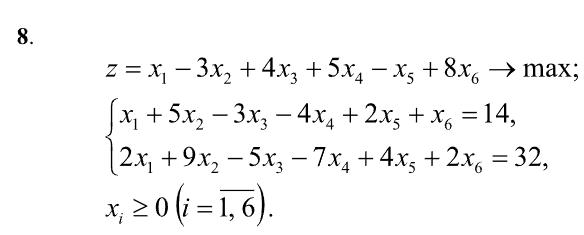
\includegraphics[width=0.75\textwidth]{uslovie.png}
\end{figure}

\newpage

\section*{Ход работы}

\subsection*{Задание 1. Изучить метод и алгоритм искусственного базиса и составить программу решения задачи ЛП этим методом}

Дана задача линейного программирования:

\[
z=x_1-3x_2+4x_3+5x_4-x_5+8x_6 \to \max
\]

при ограничениях

\[
\left\{
\begin{aligned}
x_1+5x_2-3x_3-4x_4+2x_5+x_6&=14,\\
2x_1+9x_2-5x_3-7x_4+4x_5+2x_6&=32,\\
x_i&\ge 0 \quad (i=1,\dots,6).
\end{aligned}
\right.
\]

\subsubsection*{Метод искусственного базиса (двухфазный симплекс-метод)}

Вводим искусственные переменные \(y_1\ge0,\; y_2\ge0\):

\[
\left\{
\begin{aligned}
x_1+5x_2-3x_3-4x_4+2x_5+x_6+y_1&=14,\\
2x_1+9x_2-5x_3-7x_4+4x_5+2x_6+y_2&=32.
\end{aligned}
\right.
\]

\paragraph{Фаза 1.}
Минимизируем
\[
w=y_1+y_2,
\]
или, что эквивалентно, максимизируем
\[
z_1=-w.
\]

\paragraph{Исходная симплекс-таблица.}

\[
\begin{array}{c|rrrrrrrr|r}
\text{Базис} & x_1 & x_2 & x_3 & x_4 & x_5 & x_6 & y_1 & y_2 & b\\
\hline
y_1 & 1 & 5 & -3 & -4 & 2 & 1 & 1 & 0 & 14\\
y_2 & 2 & 9 & -5 & -7 & 4 & 2 & 0 & 1 & 32\\
z_1 & -3 & -14 & 8 & 11 & -6 & -3 & 0 & 0 & -46
\end{array}
\]

\paragraph{Итерация 1.}
Самый отрицательный коэффициент в строке \(z_1\) — у переменной \(x_2\) (\(-14\)). Следовательно, ведущий столбец — \(x_2\).

Тестовые отношения:
\[
\frac{14}{5}=2.8,\qquad \frac{32}{9}\approx3.556.
\]

Минимальное отношение равно \(2.8\), значит из базиса выходит \(y_1\). Поворотный элемент равен \(5\).

Новая строка \(x_2\) (бывшая строка \(y_1\), делённая на \(5\)):

\[
\left(
\frac15,\;1,\;-\frac35,\;-\frac45,\;\frac25,\;\frac15,\;\frac15,\;0
\;\middle|\;
\frac{14}{5}
\right)
\]

Новая строка \(y_2 =\) старая строка \(y_2 - 9\) новая строка \(x_2\):

\[
\left(
\frac15,\;0,\;\frac25,\;\frac15,\;\frac25,\;\frac15,\;-\frac95,\;1
\;\middle|\;
\frac{34}{5}
\right)
\]

Новая строка \(z_1 =\) старая строка \(z_1 + 14\) новая строка \(x_2\):

\[
\left(
-\frac15,\;0,\;-\frac25,\;-\frac15,\;-\frac25,\;-\frac15,\;\frac{14}{5},\;0
\;\middle|\;
-\frac{34}{5}
\right)
\]

\paragraph{Таблица после итерации 1.}

\[
\begin{array}{c|rrrrrrrr|r}
\text{Базис} & x_1 & x_2 & x_3 & x_4 & x_5 & x_6 & y_1 & y_2 & b\\
\hline
x_2 & \frac15 & 1 & -\frac35 & -\frac45 & \frac25 & \frac15 & \frac15 & 0 & \frac{14}{5}\\
y_2 & \frac15 & 0 & \frac25 & \frac15 & \frac25 & \frac15 & -\frac95 & 1 & \frac{34}{5}\\
z_1 & -\frac15 & 0 & -\frac25 & -\frac15 & -\frac25 & -\frac15 & \frac{14}{5} & 0 & -\frac{34}{5}
\end{array}
\]

\paragraph{Итерация 2.}
Самый отрицательный коэффициент в строке \(z_1\) — у переменных \(x_3\) и \(x_5\), оба равны \(-\frac25\). Выберем ведущий столбец \(x_3\).

Тестовые отношения проводим только по положительным элементам в столбце \(x_3\):
\begin{itemize}
    \item для строки \(x_2\): коэффициент \(-\frac35<0\), не учитывается;
    \item для строки \(y_2\):
    \[
    \frac{34/5}{2/5}=17.
    \]
\end{itemize}

Следовательно, из базиса выходит \(y_2\). Поворотный элемент равен \(\frac25\).

Новая строка \(x_3\):

\[
\left(
\frac12,\;0,\;1,\;\frac12,\;1,\;\frac12,\;-\frac92,\;\frac52
\;\middle|\;
17
\right)
\]

Новая строка \(x_2 =\) старая строка \(x_2 + \frac35\) новая строка \(x_3\):

\[
\left(
\frac12,\;1,\;0,\;-\frac12,\;1,\;\frac12,\;-\frac52,\;\frac32
\;\middle|\;
13
\right)
\]

Новая строка \(z_1 =\) старая строка \(z_1 + \frac25\) новая строка \(x_3\):

\[
(0,\;0,\;0,\;0,\;0,\;0,\;1,\;1\mid 0)
\]

После этой итерации \(z_1=0\), искусственные переменные выведены из базиса. Фаза 1 завершена.

\paragraph{Таблица после фазы 1.}

\[
\begin{array}{c|rrrrrr|r}
\text{Базис} & x_1 & x_2 & x_3 & x_4 & x_5 & x_6 & b\\
\hline
x_2 & \frac12 & 1 & 0 & -\frac12 & 1 & \frac12 & 13\\
x_3 & \frac12 & 0 & 1 & \frac12 & 1 & \frac12 & 17
\end{array}
\]

\paragraph{Фаза 2.}
Переходим к исходной целевой функции
\[
z=x_1-3x_2+4x_3+5x_4-x_5+8x_6.
\]

После пересчёта строки цели получаем таблицу:

\[
\begin{array}{c|rrrrrr|r}
\text{Базис} & x_1 & x_2 & x_3 & x_4 & x_5 & x_6 & b\\
\hline
x_2 & \frac12 & 1 & 0 & -\frac12 & 1 & \frac12 & 13\\
x_3 & \frac12 & 0 & 1 & \frac12 & 1 & \frac12 & 17\\
z & \frac12 & 0 & 0 & \frac32 & -2 & \frac{15}{2} & 29
\end{array}
\]

\paragraph{Итерация 3.}
Самый положительный коэффициент в строке \(z\) — у переменной \(x_6\) \(\left(\frac{15}{2}\right)\). Следовательно, ведущий столбец — \(x_6\).

Тестовые отношения:
\[
\frac{13}{1/2}=26,\qquad \frac{17}{1/2}=34.
\]

Минимальное отношение равно \(26\), значит из базиса выходит \(x_2\). Поворотный элемент равен \(\frac12\).

Новая строка \(x_6\):
\[
(1,\;2,\;0,\;-1,\;2,\;1\mid 26)
\]

Новая строка \(x_3\):
\[
(0,\;-1,\;1,\;1,\;0,\;0\mid 4)
\]

Новая строка \(z\):
\[
(-7,\;-15,\;0,\;9,\;-17,\;0\mid 224)
\]

\paragraph{Таблица после итерации 3.}

\[
\begin{array}{c|rrrrrr|r}
\text{Базис} & x_1 & x_2 & x_3 & x_4 & x_5 & x_6 & b\\
\hline
x_6 & 1 & 2 & 0 & -1 & 2 & 1 & 26\\
x_3 & 0 & -1 & 1 & 1 & 0 & 0 & 4\\
z & -7 & -15 & 0 & 9 & -17 & 0 & 224
\end{array}
\]

\paragraph{Итерация 4.}
Самый положительный коэффициент в строке \(z\) — у переменной \(x_4\) (\(9\)). Следовательно, ведущий столбец — \(x_4\).

Тестовые отношения проводим только по положительным элементам столбца \(x_4\):
\begin{itemize}
    \item для строки \(x_6\): коэффициент \(-1<0\), не учитывается;
    \item для строки \(x_3\):
    \[
    \frac{4}{1}=4.
    \]
\end{itemize}

Из базиса выходит \(x_3\). Поворотный элемент равен \(1\).

Новая строка \(x_4\):
\[
(0,\;-1,\;1,\;1,\;0,\;0\mid 4)
\]

Новая строка \(x_6\):
\[
(1,\;1,\;1,\;0,\;2,\;1\mid 30)
\]

Новая строка \(z\):
\[
(-7,\;-6,\;-9,\;0,\;-17,\;0\mid 260)
\]

\paragraph{Оптимальная таблица.}

\[
\begin{array}{c|rrrrrr|r}
\text{Базис} & x_1 & x_2 & x_3 & x_4 & x_5 & x_6 & b\\
\hline
x_6 & 1 & 1 & 1 & 0 & 2 & 1 & 30\\
x_4 & 0 & -1 & 1 & 1 & 0 & 0 & 4\\
z & -7 & -6 & -9 & 0 & -17 & 0 & 260
\end{array}
\]

Все коэффициенты в строке целевой функции \(\le 0\), следовательно, решение оптимально.

\paragraph{Оптимальное решение.}

\[
x_4=4,\qquad x_6=30,\qquad x_1=x_2=x_3=x_5=0,
\]

\[
z^*=260.
\]

\subsection*{Задание 2. Изучить метод и алгоритм больших штрафов и составить программу решения задачи ЛП этим методом}

Вводим те же искусственные переменные \(y_1,\;y_2\) и большую константу \(M\gg0\). Тогда целевая функция принимает вид:

\[
z'=x_1-3x_2+4x_3+5x_4-x_5+8x_6-M(y_1+y_2)\to \max.
\]

Система ограничений:

\[
\left\{
\begin{aligned}
x_1+5x_2-3x_3-4x_4+2x_5+x_6+y_1&=14,\\
2x_1+9x_2-5x_3-7x_4+4x_5+2x_6+y_2&=32.
\end{aligned}
\right.
\]

Первые итерации метода больших штрафов совпадают с вычислениями Фазы 1 метода искусственного базиса: искусственные переменные выводятся из базиса, после чего дальнейшие шаги полностью соответствуют обычному симплекс-методу для исходной задачи.

Следовательно, метод больших штрафов приводит к тому же оптимальному решению:

\[
x_4=4,\qquad x_6=30,\qquad x_1=x_2=x_3=x_5=0,
\]

\[
z^*=260.
\]

\subsection*{Задание 3. Запрограммировать изученные алгоритмы и отладить соответствующие программы}

\noindent\textbf{Код программы метода искусственного базиса:}

\begin{lstlisting}
import numpy as np

EPS = 1e-10


def pivot_tableau(tableau, pivot_row_index, pivot_col_index):
    pivot_value = tableau[pivot_row_index, pivot_col_index]
    tableau[pivot_row_index, :] = tableau[pivot_row_index, :] / pivot_value

    row_count = tableau.shape[0]
    for row_index in range(row_count):
        if row_index != pivot_row_index:
            factor = tableau[row_index, pivot_col_index]
            if abs(factor) > EPS:
                tableau[row_index, :] = tableau[row_index, :] - factor * tableau[pivot_row_index, :]


def choose_entering_variable_max(tableau):
    objective_row = tableau[-1, :-1]
    entering_col_index = int(np.argmin(objective_row))
    min_value = float(objective_row[entering_col_index])

    is_optimal = True
    if min_value < -1e-12:
        is_optimal = False

    return {
        "is_optimal": is_optimal,
        "entering_col_index": entering_col_index
    }


def choose_leaving_variable(tableau, entering_col_index):
    constraint_rows = tableau[:-1, :]
    rhs_column = constraint_rows[:, -1]
    entering_column = constraint_rows[:, entering_col_index]

    leaving_row_index = -1
    best_ratio = None

    for row_index in range(constraint_rows.shape[0]):
        coefficient = entering_column[row_index]
        if coefficient > EPS:
            ratio = rhs_column[row_index] / coefficient
            if (best_ratio is None or
                    ratio < best_ratio - 1e-12 or
                    (abs(ratio - best_ratio) <= 1e-12 and row_index < leaving_row_index)):
                best_ratio = ratio
                leaving_row_index = row_index

    is_unbounded = leaving_row_index == -1
    return {
        "is_unbounded": is_unbounded,
        "leaving_row_index": leaving_row_index
    }


def simplex_maximize(tableau, basis_variable_indices, max_iterations=1000):
    status = "iter_limit"
    iteration = 0

    while iteration < max_iterations:
        entering_info = choose_entering_variable_max(tableau)

        if entering_info["is_optimal"]:
            status = "optimal"
            break

        entering_col_index = entering_info["entering_col_index"]
        leaving_info = choose_leaving_variable(tableau, entering_col_index)

        if leaving_info["is_unbounded"]:
            status = "unbounded"
            break

        leaving_row_index = leaving_info["leaving_row_index"]
        pivot_tableau(tableau, leaving_row_index, entering_col_index)
        basis_variable_indices[leaving_row_index] = entering_col_index

        iteration += 1

    return {
        "status": status,
        "tableau": tableau,
        "basis": basis_variable_indices
    }


def build_phase1_tableau_with_artificial(A_matrix, rhs_vector):
    constraint_count, variable_count = A_matrix.shape
    artificial_identity = np.eye(constraint_count)

    augmented_matrix = np.hstack([A_matrix.astype(float), artificial_identity])
    total_variable_count = variable_count + constraint_count

    tableau = np.zeros((constraint_count + 1, total_variable_count + 1), dtype=float)
    tableau[:constraint_count, :total_variable_count] = augmented_matrix
    tableau[:constraint_count, -1] = rhs_vector.astype(float)

    phase1_cost = np.zeros(total_variable_count, dtype=float)
    phase1_cost[variable_count:] = -1.0

    basis_variable_indices = [variable_count + i for i in range(constraint_count)]

    basis_costs = phase1_cost[basis_variable_indices]
    tableau[-1, :total_variable_count] = (
        basis_costs @ tableau[:constraint_count, :total_variable_count]
    ) - phase1_cost
    tableau[-1, -1] = basis_costs @ tableau[:constraint_count, -1]

    return {
        "tableau": tableau,
        "basis": basis_variable_indices,
        "original_variable_count": variable_count
    }


def try_remove_artificials_from_basis(tableau, basis_variable_indices, original_variable_count):
    constraint_count = tableau.shape[0] - 1

    for row_index in range(constraint_count):
        basis_index = basis_variable_indices[row_index]
        if basis_index >= original_variable_count:
            pivoted = False
            for col_index in range(original_variable_count):
                if abs(tableau[row_index, col_index]) > EPS:
                    pivot_tableau(tableau, row_index, col_index)
                    basis_variable_indices[row_index] = col_index
                    pivoted = True
                    break
            if not pivoted:
                pass


def build_phase2_tableau(phase1_tableau, phase1_basis, objective_cost, original_variable_count):
    constraint_count = phase1_tableau.shape[0] - 1

    tableau = np.zeros((constraint_count + 1, original_variable_count + 1), dtype=float)
    tableau[:constraint_count, :original_variable_count] = \
        phase1_tableau[:constraint_count, :original_variable_count]
    tableau[:constraint_count, -1] = phase1_tableau[:constraint_count, -1]

    basis_variable_indices = list(phase1_basis)

    basis_ok = True
    for row_index in range(constraint_count):
        if basis_variable_indices[row_index] >= original_variable_count:
            basis_ok = False

    if basis_ok:
        basis_costs = objective_cost[basis_variable_indices]
        tableau[-1, :original_variable_count] = (
            basis_costs @ tableau[:constraint_count, :original_variable_count]
        ) - objective_cost
        tableau[-1, -1] = basis_costs @ tableau[:constraint_count, -1]

    return {
        "tableau": tableau,
        "basis": basis_variable_indices,
        "basis_ok": basis_ok
    }


def extract_solution(tableau, basis_variable_indices, variable_count):
    solution = np.zeros(variable_count, dtype=float)
    constraint_count = tableau.shape[0] - 1

    for row_index in range(constraint_count):
        basis_var = basis_variable_indices[row_index]
        if basis_var < variable_count:
            solution[basis_var] = tableau[row_index, -1]

    objective_value = float(tableau[-1, -1])
    return {
        "x": solution,
        "z": objective_value
    }


def solve_two_phase(A_matrix, rhs_vector, objective_cost):
    status = "unknown"
    solution_vector = None
    objective_value = None

    phase1_data = build_phase1_tableau_with_artificial(A_matrix, rhs_vector)
    phase1_result = simplex_maximize(phase1_data["tableau"], phase1_data["basis"])

    phase1_status = phase1_result["status"]
    phase1_tableau = phase1_result["tableau"]
    phase1_basis = phase1_result["basis"]
    original_variable_count = phase1_data["original_variable_count"]

    if phase1_status != "optimal":
        status = phase1_status
    else:
        phase1_objective = float(phase1_tableau[-1, -1])

        feasible = abs(phase1_objective) <= 1e-8
        if not feasible:
            status = "infeasible"
        else:
            try_remove_artificials_from_basis(
                phase1_tableau,
                phase1_basis,
                original_variable_count
            )

            phase2_data = build_phase2_tableau(
                phase1_tableau,
                phase1_basis,
                objective_cost.astype(float),
                original_variable_count
            )

            if not phase2_data["basis_ok"]:
                status = "infeasible"
            else:
                phase2_result = simplex_maximize(
                    phase2_data["tableau"],
                    phase2_data["basis"]
                )

                status = phase2_result["status"]

                if status == "optimal":
                    solution_data = extract_solution(
                        phase2_result["tableau"],
                        phase2_result["basis"],
                        original_variable_count
                    )
                    solution_vector = solution_data["x"]
                    objective_value = solution_data["z"]

    return {
        "status": status,
        "x": solution_vector,
        "z": objective_value
    }


def main():
    A_matrix = np.array([
        [1, 5, -3, -4, 2, 1],
        [2, 9, -5, -7, 4, 2]
    ], dtype=float)

    rhs_vector = np.array([14, 32], dtype=float)

    objective_cost = np.array([1, -3, 4, 5, -1, 8], dtype=float)

    result = solve_two_phase(A_matrix, rhs_vector, objective_cost)

    print("Метод искусственного базиса")
    print("Статус:", result["status"])
    if result["status"] == "optimal":
        print("x:", np.round(result["x"], 6))
        print("z:", round(result["z"], 6))


if __name__ == "__main__":
    main()
\end{lstlisting}

\text{Результат работы:}

\begin{figure}[H]
    \centering
    \includegraphics[width=0.75\textwidth]{result1.png}
    \text{Рис.1: Результат работы программы для метода искусственного базиса.}
\end{figure}

\text{Блок-схемы метода искусственного базиса:}

\begin{figure}[H]
    \centering
    
\includegraphics[width=0.75\textwidth]{MainProg.png}
    \text{Рис.2: Блок-схема main.}
\end{figure}

\begin{figure}[H]
    \centering
    
\includegraphics[width=1.0\textwidth]{defPivot_tableau.png}
    \text{Рис.3: Блок-схема функции pivot\_tableau.}
\end{figure}

\begin{figure}[H]
    \centering
    
\includegraphics[width=0.75\textwidth]{def choose_entering_variable_max.png}
    \text{Рис.4: Блок-схема функции choose\_entering\_variable\_max.}
\end{figure}

\begin{figure}[H]
    \centering
    
\includegraphics[width=0.9\textwidth]{def choose_leaving_variable.png}
    \text{Рис.5: Блок-схема функции choose\_leaving\_variable.}
\end{figure}

\begin{figure}[H]
    \centering
    
\includegraphics[width=0.75\textwidth]{def simplex_maximizePart1.png}
    \text{Рис.6: Блок-схема функции simplex\_maximize.}
\end{figure}

\begin{figure}[H]
    \centering
    
\includegraphics[width=0.75\textwidth]{def simplex_maximizePart2.png}
    \text{Рис.7: Продолжение блок-схемы функции simplex\_maximize.}
\end{figure}

\begin{figure}[H]
    \centering
    
\includegraphics[width=0.75\textwidth]{def build_phase1_tableau_with_artificial.png}
    \text{Рис.8: Блок-схема функции build\_phase1\_tableau\_with\_artificial.}
\end{figure}

\begin{figure}[H]
    \centering
    
\includegraphics[width=0.9\textwidth]{def try_remove_artificials_from_basis.png}
    \text{Рис.9: Блок-схема функции try\_remove\_artificials\_from\_basis.}
\end{figure}

\begin{figure}[H]
    \centering
    
\includegraphics[width=1.0\textwidth]{def build_phase2_tableau.png}
    \text{Рис.10: Блок-схема функции build\_phase2\_tableau.}
\end{figure}

\begin{figure}[H]
    \centering
    
\includegraphics[width=1.0\textwidth]{def extract_solution.png}
    \text{Рис.11: Блок-схема функции extract\_solution.}
\end{figure}

\begin{figure}[H]
    \centering
    
\includegraphics[width=0.75\textwidth]{def solve_two_phasePart1.png}
    \text{Рис.12: Блок-схема функции solve\_two\_phase.}
\end{figure}

\begin{figure}[H]
    \centering
    
\includegraphics[width=0.75\textwidth]{def solve_two_phasePart2.png}
    \text{Рис.13: Продолжение блок-схемы функции solve\_two\_phase.}
\end{figure}

\begin{figure}[H]
    \centering
    
\includegraphics[width=0.75\textwidth]{def main.png}
    \text{Рис.14: Блок-схема функции main.}
\end{figure}

\text{Код программы метода больших штрафов:}

\begin{lstlisting}
import numpy as np

EPS = 1e-10


def pivot_tableau(tableau, pivot_row_index, pivot_col_index):
    pivot_value = tableau[pivot_row_index, pivot_col_index]
    tableau[pivot_row_index, :] = tableau[pivot_row_index, :] / pivot_value

    row_count = tableau.shape[0]
    for row_index in range(row_count):
        if row_index != pivot_row_index:
            factor = tableau[row_index, pivot_col_index]
            if abs(factor) > EPS:
                tableau[row_index, :] = tableau[row_index, :] - factor * tableau[pivot_row_index, :]


def choose_entering_variable_max(tableau):
    objective_row = tableau[-1, :-1]
    entering_col_index = int(np.argmin(objective_row))
    min_value = float(objective_row[entering_col_index])

    is_optimal = True
    if min_value < -1e-12:
        is_optimal = False

    return {
        "is_optimal": is_optimal,
        "entering_col_index": entering_col_index
    }


def choose_leaving_variable(tableau, entering_col_index):
    constraint_rows = tableau[:-1, :]
    rhs_column = constraint_rows[:, -1]
    entering_column = constraint_rows[:, entering_col_index]

    leaving_row_index = -1
    best_ratio = None

    for row_index in range(constraint_rows.shape[0]):
        coefficient = entering_column[row_index]
        if coefficient > EPS:
            ratio = rhs_column[row_index] / coefficient
            if (best_ratio is None or
                    ratio < best_ratio - 1e-12 or
                    (abs(ratio - best_ratio) <= 1e-12 and row_index < leaving_row_index)):
                best_ratio = ratio
                leaving_row_index = row_index

    is_unbounded = leaving_row_index == -1
    return {
        "is_unbounded": is_unbounded,
        "leaving_row_index": leaving_row_index
    }


def simplex_maximize(tableau, basis_variable_indices, max_iterations=1000):
    status = "iter_limit"
    iteration = 0

    while iteration < max_iterations:
        entering_info = choose_entering_variable_max(tableau)

        if entering_info["is_optimal"]:
            status = "optimal"
            break

        entering_col_index = entering_info["entering_col_index"]
        leaving_info = choose_leaving_variable(tableau, entering_col_index)

        if leaving_info["is_unbounded"]:
            status = "unbounded"
            break

        leaving_row_index = leaving_info["leaving_row_index"]
        pivot_tableau(tableau, leaving_row_index, entering_col_index)
        basis_variable_indices[leaving_row_index] = entering_col_index

        iteration += 1

    return {
        "status": status,
        "tableau": tableau,
        "basis": basis_variable_indices
    }


def extract_solution(tableau, basis_variable_indices, variable_count):
    solution = np.zeros(variable_count, dtype=float)
    constraint_count = tableau.shape[0] - 1

    for row_index in range(constraint_count):
        basis_var = basis_variable_indices[row_index]
        if basis_var < variable_count:
            solution[basis_var] = tableau[row_index, -1]

    return {
        "x": solution,
        "z": float(tableau[-1, -1])
    }


def solve_big_m(A_matrix, rhs_vector, objective_cost, big_m_value=1e6):
    status = "unknown"
    solution_vector = None
    objective_value = None

    constraint_count, variable_count = A_matrix.shape
    artificial_identity = np.eye(constraint_count)

    augmented_matrix = np.hstack([A_matrix.astype(float), artificial_identity])
    augmented_cost = np.concatenate([
        objective_cost.astype(float),
        -big_m_value * np.ones(constraint_count)
    ])

    total_variable_count = variable_count + constraint_count

    tableau = np.zeros((constraint_count + 1, total_variable_count + 1), dtype=float)
    tableau[:constraint_count, :total_variable_count] = augmented_matrix
    tableau[:constraint_count, -1] = rhs_vector.astype(float)

    basis_variable_indices = [variable_count + i for i in range(constraint_count)]

    basis_costs = augmented_cost[basis_variable_indices]
    tableau[-1, :total_variable_count] = (
        basis_costs @ tableau[:constraint_count, :total_variable_count]
    ) - augmented_cost
    tableau[-1, -1] = basis_costs @ tableau[:constraint_count, -1]

    simplex_result = simplex_maximize(tableau, basis_variable_indices)

    status = simplex_result["status"]
    final_tableau = simplex_result["tableau"]
    final_basis = simplex_result["basis"]

    if status == "optimal":
        extended_solution = np.zeros(total_variable_count, dtype=float)
        for row_index in range(constraint_count):
            extended_solution[final_basis[row_index]] = final_tableau[row_index, -1]

        artificial_part = extended_solution[variable_count:]
        infeasible = np.max(np.abs(artificial_part)) > 1e-8

        if infeasible:
            status = "infeasible"
        else:
            solution_vector = extended_solution[:variable_count]
            objective_value = float(objective_cost @ solution_vector)

    return {
        "status": status,
        "x": solution_vector,
        "z": objective_value
    }


def main():
    A_matrix = np.array([
        [1, 5, -3, -4, 2, 1],
        [2, 9, -5, -7, 4, 2]
    ], dtype=float)

    rhs_vector = np.array([14, 32], dtype=float)

    objective_cost = np.array([1, -3, 4, 5, -1, 8], dtype=float)

    result = solve_big_m(A_matrix, rhs_vector, objective_cost, big_m_value=1e6)

    print("Метод больших штрафов")
    print("Статус:", result["status"])
    if result["status"] == "optimal":
        print("x:", np.round(result["x"], 6))
        print("z:", round(result["z"], 6))


if __name__ == "__main__":
    main()
\end{lstlisting}

\text{Результат работы программы:}

\begin{figure}[H]
    \centering
    
\includegraphics[width=0.75\textwidth]{result2.png}
    \text{Рис.15: Результат работы программы для метода больших штрафов.}
\end{figure}

\text{Блок-схемы метода больших штрафов:}

\begin{figure}[H]
    \centering
    
\includegraphics[width=0.75\textwidth]{Main2.png}
    \text{Рис.16: Блок-схема функции main.}
\end{figure}

\begin{figure}[H]
    \centering
    
\includegraphics[width=1.0\textwidth]{def pivot_tableau2.png}
    \text{Рис.17: Блок-схема функции pivot\_tableau.}
\end{figure}

\begin{figure}[H]
    \centering
    
\includegraphics[width=0.75\textwidth]{def choose_entering_variable_max2.png}
    \text{Рис.18: Блок-схема функции choose\_entering\_variable\_max.}
\end{figure}

\begin{figure}[H]
    \centering
    
\includegraphics[width=1.0\textwidth]{def choose_leaving_variable2.png}
    \text{Рис.19: Блок-схема функции choose\_leaving\_variable.}
\end{figure}

\begin{figure}[H]
    \centering
    
\includegraphics[width=0.75\textwidth]{def simplex_maximize2Part1.png}
    \text{Рис.20: Блок-схема функции simplex\_maximize.}
\end{figure}

\begin{figure}[H]
    \centering
    
\includegraphics[width=0.75\textwidth]{def simplex_maximize2Part2.png}
    \text{Рис.21: Продолжение блок-схемы функции simplex\_maximize.}
\end{figure}

\begin{figure}[H]
    \centering
    
\includegraphics[width=0.75\textwidth]{def extract_solution2.png}
    \text{Рис.22: Блок-схема функции extract\_solution.}
\end{figure}

\begin{figure}[H]
    \centering
    
\includegraphics[width=1.0\textwidth]{def solve_big_m2Part1.png}
    \text{Рис.23: Блок-схема функции solve\_big\_m.}
\end{figure}

\begin{figure}[H]
    \centering
    
\includegraphics[width=0.75\textwidth]{def solve_big_m2Part2.png}
    \text{Рис.24: Продолжение блок-схемы функции solve\_big\_m.}
\end{figure}

\section*{Вывод}

В ходе выполнения лабораторной работы были изучены два метода решения задач линейного программирования в канонической форме, не имеющих готового допустимого базисного решения: метод искусственного базиса и метод больших штрафов. Были подробно разобраны принципы построения начальной симплекс-таблицы с введением искусственных переменных, алгоритмы выполнения первой и второй фаз двухфазного метода, а также механизм учёта большого штрафа \(M\) в целевой функции. Особое внимание уделялось правилам выбора разрешающего элемента, выполнению pivot-преобразований и проверке условий оптимальности и допустимости решения.

На основе изученных алгоритмов были разработаны и отлажены программы на языке Python, реализующие оба метода. Программы разбиты на небольшие функциональные блоки, что позволило наглядно представить их в виде блок-схем.

Таким образом, поставленная цель работы достигнута: получены теоретические знания и практические навыки применения методов искусственного базиса и больших штрафов, а также опыт разработки, отладки и тестирования соответствующих алгоритмов.

\end{document}